\documentclass[a4,10pt]{book}
\addtolength{\textwidth}{1in}
\addtolength{\hoffset}{-0.5in}
\addtolength{\textheight}{1in}
\addtolength{\voffset}{-0.5in}
\usepackage{natbib}
\usepackage{setspace}
\usepackage{amsmath}
\usepackage{amssymb}
\usepackage{graphicx}
\usepackage{fancyhdr}
\usepackage{mathrsfs}
\usepackage{makeidx}
\usepackage{color}

\newtheorem{definition}[section]{Definition}
\newtheorem{theorem}[section]{Theorem}
\renewcommand{\textfraction}{0.05}
\makeindex
\title{Hotelling's T$^{2}$}
\author{Paul J. Hewson}
\onehalfspacing
%\address{ School of Mathematics and Statistics, University of Plymouth, Drake Circus, Plymouth PL4 8AA, UK}
%\email{paul.hewson@plymouth.ac.uk}

\begin{document}
\frontmatter
\setlength{\parindent}{0pt}
\setlength{\parskip}{12pt}

\newcommand{\R}{\textbf{\color{blue}{R}\ }}
\pagestyle{fancy}
\lhead{Hotellings}
\chead{}
\rhead{}
\lfoot{}
\cfoot{\copyright Paul Hewson}
\rfoot{\thepage}
\renewcommand{\headrulewidth}{0.4pt}
\renewcommand{\footrulewidth}{0.4pt}

\sffamily
\maketitle

\mainmatter

\chapter{Inference for the mean}
\label{meaninf}


We introduced the Mahalanobis distance earlier in \ref{standarddist}.   Consideration of the \emph{squared} Mahalabnobis distance leads us to consider the so called T$^{2}$ statistic (the nomenclature reflects that this relates to a $t$-statistic for one variable). This can be found as:

\begin{equation}
\label{t2}
T^{2} = n (\boldsymbol{\mu}_{0} - \bar{\boldsymbol{x}})^{T} \boldsymbol{S}  (\boldsymbol{\mu}_{0} - \bar{\boldsymbol{x}})
\end{equation}
where $n$ is the sample size, $\boldsymbol{\mu}_{0}$ is the hypothesised mean, $\bar{\boldsymbol{x}}$ and $\boldsymbol{S}$ are the sample mean and covariance matrices respectively.    It turns out that this statistic follows a T$^{2}$ distribution, however, given that there is a simple relationship between the T$^{2}$ and $F$ distribution it is often easier to work with the latter.


%turn this into a theorm ala flury 379, proof in Anderson and Seber (and muirhead
If $\boldsymbol{x}_{i}$, $i = 1, \ldots n$ represent a sample from a $p$ variate normal distribution with mean $\boldsymbol{\mu}$ and covariance $\boldsymbol{\Sigma}$, provided $\boldsymbol{\Sigma}$ is positive definite and $n > p$, given sample estimators for mean and covariance $\bar{\boldsymbol{x}}$ and $\boldsymbol{S}$ respectively, then:
\begin{equation}
F = \left(\frac{n}{n-1}\right) \left(\frac{n-p}{p}\right)  (\boldsymbol{\mu}_{0} - \bar{\boldsymbol{x}})^{T} \boldsymbol{S}  (\boldsymbol{\mu}_{0} - \bar{\boldsymbol{x}})
\end{equation}
follows an $F$-distribution with $p$ and $(n-p)$ degrees of freedom.   Note the requirement that $n > p$, i.e. that $\boldsymbol{S}$ is non-singular.   This clearly limits the use of this test in bio-informatic applications and we may examine a few proposals to deal with this.   To carry out a test on $\boldsymbol{\mu}$, we determine whether $F \leq F_{(1-\alpha),p,n-p}$, the $(1-\alpha)$ quantile of the $F$ distribution on $p$ and $n-p$ degrees of freedom.   We reject the null hypothesis if our test statistic exceeds this value.   We will not consider the one sample T$^{2}$ test any further, but will now examine the two-sampled test.

\section{Two sample Hotelling's T$^{2}$  test}
\label{t2}

Analagous to the univariate context, we wish to determine whether the mean vectors are comparable, more formally:
\begin{equation}
H_{0}: \boldsymbol{\mu}_{1} = \boldsymbol{\mu}_{2}
\end{equation}

The T$^{2}$ statistic proposed by \cite{Hotelling:1931}, will be based this time on the distance between two mean vectors.   It can be calculated as:

\begin{equation}
\label{hotelling}
T^{2} = \left(\frac{n_{1}n_{2}}{n_{1}+n_{2}}\right)(\boldsymbol{\bar{x}_{1}} - \boldsymbol{\bar{x}_{2}})^{T}\boldsymbol{S}^{-1}(\boldsymbol{\bar{x}_{1}} - \boldsymbol{\bar{x}_{2}})
\end{equation}
where $S^{-1}$ is the inverse of the pooled correlation matrix given by:
\begin{displaymath}
\label{poolcov}
\boldsymbol{S} = \frac{(n_{1} - 1) \boldsymbol{S_{1}} + (n_{2} - 1) \boldsymbol{S_{2}}}{n_{1} + n_{2} - 2}
\end{displaymath}
given the sample estimates for covariance, $\boldsymbol{S_{1}}$ and $\boldsymbol{S_{2}}$ in the two samples.   As before, there is a simple relationship between the test statistic, $T^2$, and the $F$ distribution.   

%make theorm flury 404, proof seber, anderson
If $\boldsymbol{x}_{1i}$, $i = 1, \ldots n_{1}$ and $\boldsymbol{x}_{2i}$, $i = 1, \ldots n_{2}$ represent independent samples from two $p$ variate normal distribution with mean vectors $\boldsymbol{\mu}_{1}$ and  $\boldsymbol{\mu}_{2}$ but with common covariance matrix $\boldsymbol{\Sigma}$, provided $\boldsymbol{\Sigma}$ is positive definite and $n > p$, given sample estimators for mean and covariance $\bar{\boldsymbol{x}}$ and $\boldsymbol{S}$ respectively, then:
\begin{displaymath}
F = \frac{(n_{1} + n_{2} - p - 1) T^{2}}{(n_{1} + n_{2} - 2)p}
\end{displaymath}
has an $F$ distribution on $p$ and $(n_{1}+n_{2}-p-1)$ degrees of freedom.   Essentially, we compute the test statistic, and see whether it falls within the $(1-\alpha)$ quantile of the F distribution on those degrees of freedom.   note again that to ensure non-singularity of $\boldsymbol{S}$, we require that $n_{1}+n_{2} > p$.

Whilst we won't use the next formula for computation, it may clarify understanding of this test if we consider the sample estimate of the mean difference $\boldsymbol{d} = \bar{\boldsymbol{x}}_{1} - \bar{\boldsymbol{x}}_{2}$, and the corresponding population distance $\boldsymbol{\delta} = \boldsymbol{\mu}_{1} - \boldsymbol{\mu}_{2}$ we can use the formula:
\begin{displaymath}
F = \left( \frac{n_{1} + n_{2} - p - 1}{p(n_{1} + n_{2} - 2)} \right) \left(\frac{n_{1}n_{2}}{n_{1}+n_{2}} \right) (\boldsymbol{d} - \boldsymbol{\delta})^{T}\boldsymbol{S}^{-1}(\boldsymbol{d} - \boldsymbol{\delta})
\end{displaymath}
to calculate the test statistic. 




We are going to consider an example using data from Flea Beetles reported by \cite{Lubischew:1962} and used in [page 307] \cite{Flury:1997}.   It should be noted that in terms of practical computation, methods are based on the QR decomposition will be used, details are given in \cite{Seber:1984}.   However, for the purposes of understanding the principles behind the test, we follow the formula directly.


\singlespacing
\begin{verbatim}
> library(Flury)
> ?flea.beetles
> data(flea.beetles)
\end{verbatim}
\onehalfspacing

It can be seen that there is a factor ``Species'' denoting whether the beetles are from 'oleracea' or 'carduorum'.   There are four numeric variables as follows: 'TG'; Distange of the Transverse Groove to the posterior border of
          the prothorax (microns), 'Elytra'; Length of the Elytra (in units of 0.01mm), 'Second.Antenna'; Length of the second antennal joint (microns) and 'Third.Antenna'; Length of the third antennal joint (microns).   We need to estimate the mean for each sample, and calculate the difference between the two vectors:
\singlespacing
\begin{verbatim}
mu <- by(flea.beetles[,-1], flea.beetles$Species, colMeans)
mudiff <- mu[[1]] - mu[[2]]
p <- dim(flea.beetles)[2] - 1 ## how many variables are we using
\end{verbatim}
\onehalfspacing

The next step is to extract the two covariance matrices:

\singlespacing
\begin{verbatim}
> covmats <- by(flea.beetles[,-1], flea.beetles$Species, cov)
> covmats
\end{verbatim}
\onehalfspacing
and then to estimate the pooled covariance matrix $\boldsymbol{S}$ for the flea beetle data (where N[1] gives $n_{1}$,  N[2] gives $n_{2}$), can be calculated as:

\singlespacing
\begin{verbatim}
> N <- xtabs(~flea.beetles[,1])
> pooledS <- ((N[1]-1) * covmats[[1]] + (N[2]-1) * covmats[[2]]) / (N[1] + N[2] -2)
> pooledS
> Sinv <- solve(pooledS)
> Sinv
                         TG        Elytra Second.Antenna Third.Antenna
TG              0.013257964 -0.0053492256   0.0015134494 -0.0021617878
Elytra         -0.005349226  0.0066679441  -0.0047337699 -0.0005969439
Second.Antenna  0.001513449 -0.0047337699   0.0130490933 -0.0007445297
Third.Antenna  -0.002161788 -0.0005969439  -0.0007445297  0.0060093005
\end{verbatim}
\onehalfspacing

Having calculated the inverse of the pooled correlation matrix we also need the scaling factor $\frac{n_{1} n_{2}}{n_{1} + n_{2}}$.   Hotellings T$^{2}$ is then quite straightforward to calculate:


\singlespacing
\begin{verbatim}
> scaleFact <- (N[1]*N[2]) / (N[1]+N[2])
> Hotellings <-  t(mudiff) %*% Sinv %*% mudiff * scaleFact
> Hotellings
         [,1]
[1,] 133.4873
\end{verbatim}
\onehalfspacing
which is the value of the T$^{2}$ statistic.   We could work with this value directly, but it is more convenient to transform it into something we can compare with the $F$ distribution.
\singlespacing
\begin{verbatim}
test <- ((N[1] + N[2] - p - 1) * Hotellings )/ ((N[1] + N[2] - 2) * p)
test
       [,1]
[1,] 30.666
\end{verbatim}
\onehalfspacing

and we compare this with an $F$ distribution having $p$ and $(n_{1} + n_{2} - p - 1)$ d.f.

And we can check this as follows:
\singlespacing
\begin{verbatim}
> pf(test, p, N[1]+N[2]-p-1,lower.tail = FALSE )
             [,1]
[1,] 3.215324e-11
\end{verbatim}
\onehalfspacing
which gives us the area under the curve from our test statistic ($30.666$) to $\infty$.   Clearly in this case, we have reject H$_{0}$, i.e. there is evidence that the mean vectors, $\bar{\boldsymbol{x}}_{oleracea} = (194.4737, 267.0526, 137.3684, 185.9474), \bar{\boldsymbol{x}}_{carduorum} = (179.55, 290.80, 157.20, 209.25)$, 
 for the two species differ.   This is perhaps no surprise if you consider the data.   Figure \ref{lubishew} contains a scatterplot where different symbols have been used in the lower panels for the two species.   However, we do need to consider this in a little more detail.  

\begin{figure}
\begin{center}
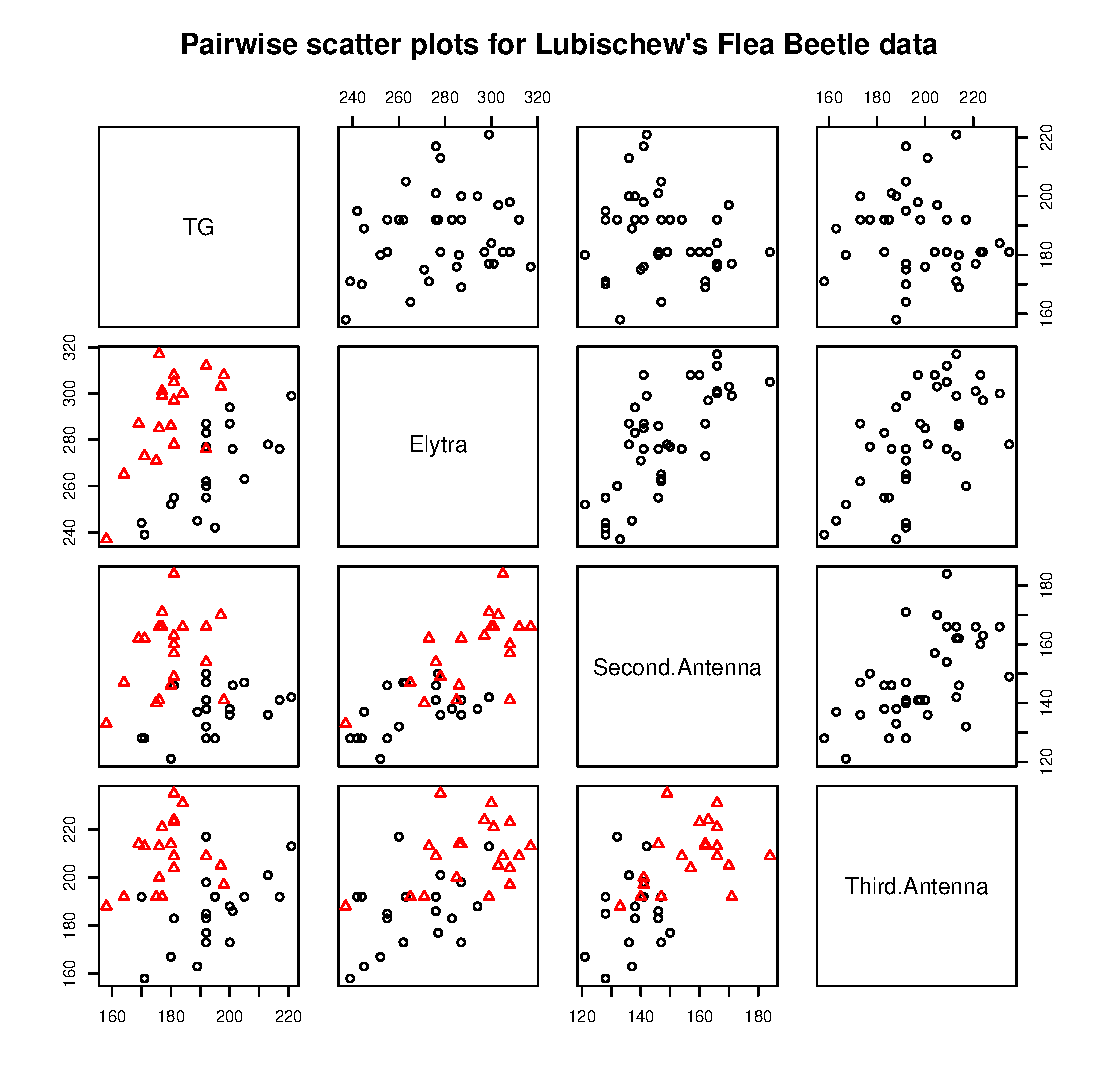
\includegraphics[width = 0.6\textwidth]{images/lubishew}
\caption{Scatterplot for Lubischew flea data, lower panel has symbols denoting the two species}
\label{lubishew}
\end{center}
\end{figure}



\section{Constant Density Ellipses}
\label{cdellipse}

\cite{Flury:1997} gives an interpretation of constant density ellipses in terms of the Mahalanobis distance which is worth reading.   Essentially, we wish to find a region of squared Mahlanobis distance such that:
\begin{displaymath}
Pr \left( (\boldsymbol{\bar{x}} - \boldsymbol{\mu})^{T} \boldsymbol{S}^{-1} (\boldsymbol{\bar{x}} - \boldsymbol{\mu}) \right) c^{2}) 
\end{displaymath}
and we can find $c^{2}$ as follows:
\begin{displaymath}
c^{2} = \left( \frac{n-1}{n} \right) \left( \frac{p}{n-p} \right) F_{(1-\alpha), p, (n-p)}
\end{displaymath}
where $F_{(1-\alpha), p, (n-p)}$ is the $(1-\alpha)$ quantile of the $F$ distribution with $p$ and $n-p$ degrees of freedom, $p$ represents the number of variables and $n$ the sample size.


This illustration is based on, but differs from code provided by Marco Bee to accompany and will make much more sense if used in conjunction with that book.   It is worth checking how and why this code differs!   Firstly, we need a function to draw ellipses:

\singlespacing
\begin{verbatim}
ellipse <- function(covmat, centroid, csquare, resolution, plot = TRUE) {
angles <- seq(0, by = (2 * pi)/resolution, length = resolution)
  sd <- covmat[1,2] / sqrt(covmat[1,1] * covmat[2,2])
    projmat <- matrix(0,2,2)
    projmat[1,1] <- sqrt(covmat[1,1] %*% (1+sd)/2)
    projmat[1,2] <- -sqrt(covmat[1,1] %*% (1-sd)/2)
    projmat[2,1] <- sqrt(covmat[2,2] %*% (1+sd)/2)
    projmat[2,2] <- sqrt(covmat[2,2] %*% (1-sd)/2)
circle <- cbind(cos(angles), sin(angles))
ellipse <- t(centroid + sqrt(csquare) * projmat %*% t(circle))
if (plot == TRUE) {lines(ellipse)}
return(ellipse)
}
\end{verbatim}
\onehalfspacing

It is possible to define a function which calculates $c^{2}$ and calls the ellipse routine (I'm not completely convinced this is doing the calculation correctly yet, in particular I'm not sure I'm using the correct tail).

\singlespacing
\begin{verbatim}
function (data, alpha=0.05, resolution=500) 
{
xbar <- colMeans(data)
n <- dim(data)[1]
p <- dim(data)[2]
f <- qf(1-alpha, p, n-p)
csquare <- ((n-1)/n) * (p / (n-p)) * f
cat(csquare) 
ellipse <- ellipse(cov(data), xbar, csquare, resolution)
}
\end{verbatim}
\onehalfspacing

%# call procedure ellips

%X <- ellips(A, m, const, k)               

%# graph the results

For illustrative purposes, we'll create a $n \times 2$ data object from our flea beetles, and plot the confidence ellipse for these.

\singlespacing
\begin{verbatim}
X <- cbind(flea.beetles[,2], flea.beetles[,3])
plot(X)
cdellipse(X, alpha = 0.01)
cdellipse(X, alpha = 0.05)
\end{verbatim}
\onehalfspacing


These can be contrasted with the univariate confidence intervals:

\singlespacing
\begin{verbatim}
abline(v = confint(lm(X[,1]~1)))
abline(h = confint(lm(X[,2]~1)))
\end{verbatim}
\onehalfspacing

This exercise should be repeated with the turtles data!   However, it is possible to illustrate the basic idea with the sibling heads data, where we construct two derivative variables indicating the difference in head breadth and the difference in head width.   These are plotted in figure \ref{cdellipse}, it can be seen that the univariate confidence intervals and the constant density ellipse support different areas of parameter space.   Ignoring the correlation structure in these data could lead to flaws in inference when assessesing parameter uncertainty.

\begin{figure}
\begin{center}
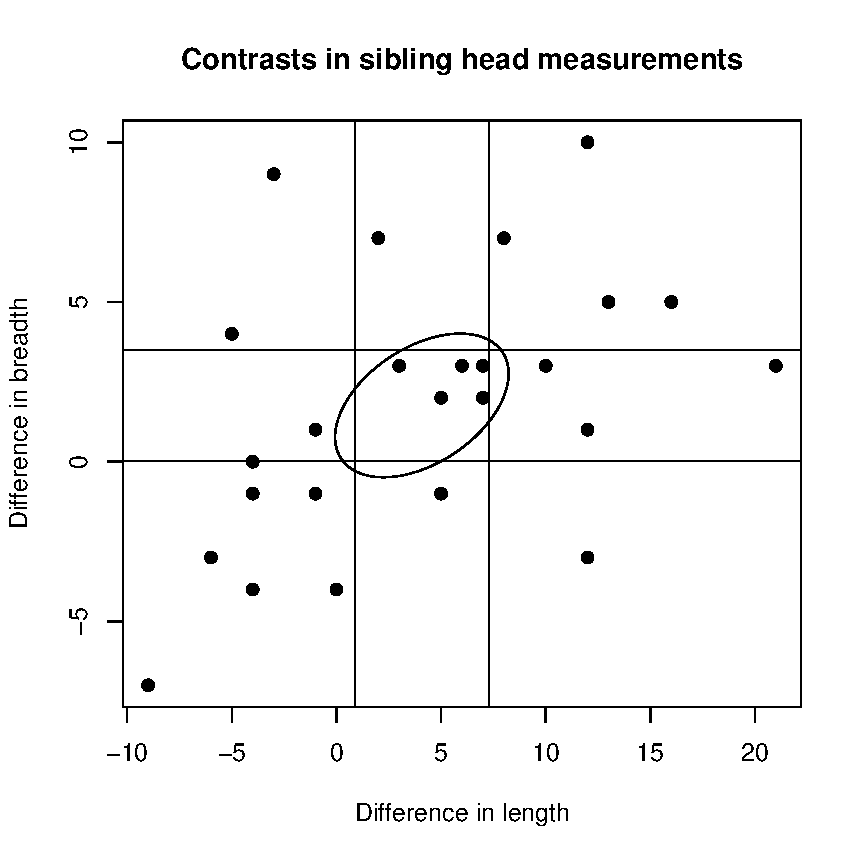
\includegraphics[width = 0.5\textwidth]{images/cdellipse}
\caption{Constant density ellipse for mean vector for difference in head width and breadth, and univariate confidence intervals for the mean of each variable}
\label{cdellipse}
\end{center}
\end{figure}



% X <- sibling.heads
%Y <- cbind((X[, 1] - X[, 3]),(X[, 2] - X[, 4]))
%plot(Y, main = "Contrasts in sibling head measurements", xlab = "Difference in length", ylab = "Difference in breadth", pch = 16)
%X <- Y
%cdellipse(X)
%abline(v = confint(lm(X[,1]~1)))
%abline(h = confint(lm(X[,2]~1)))


%\section{Likelihood ratio tests}
%\label{lrt}

%\section{Profile analysis}
%\label{profile}

%\section{Confidence regions}
%\label{confR}

%\section{Multivariate analysis of variance}
%\label{manova}

%\section{Multivariate regression}
%\label{mvreg}

%\section{Shrinkage of parameters in multivariate regression}
%\label{shrinkage}

%\section{Introduction to the forward search}
%\label{forward}

\section{Multivariate Analysis of Variance}
\label{manova}

As with the univariate situation, t-tests are fine for comparing the means of two groups, but we would have ``multiple comparison'' problems if we tried to compare more than two.   In an analagous way, in the multivariate context we have MANOVA.

First of all we'll enter some data relating to the production of plastic film reported in \cite{Krzanowski:2000}.   Tear, gloss and opacity are measures of the manufactured films.

\singlespacing
\begin{verbatim}
> tear <- c(6.5, 6.2, 5.8, 6.5, 6.5, 6.9, 7.2, 6.9, 6.1, 6.3,                
            6.7, 6.6, 7.2, 7.1, 6.8, 7.1, 7.0, 7.2, 7.5, 7.6)
> gloss <- c(9.5, 9.9, 9.6, 9.6, 9.2, 9.1, 10.0, 9.9, 9.5, 9.4,
             9.1, 9.3, 8.3, 8.4, 8.5, 9.2, 8.8, 9.7, 10.1, 9.2)
> opacity <- c(4.4, 6.4, 3.0, 4.1, 0.8, 5.7, 2.0, 3.9, 1.9, 5.7,
               2.8, 4.1, 3.8, 1.6, 3.4, 8.4, 5.2, 6.9, 2.7, 1.9)
Y <- cbind(tear, gloss, opacity)
\end{verbatim}
\onehalfspacing

We now need to put in information on the rate of extrusion, and the amount of additive used (\texttt{gl()} is a command which specifically creates these kind of experimental factors).

\singlespacing
\begin{verbatim}
> rate <- factor(gl(2,10), labels=c("Low", "High"))
> additive <- factor(gl(2, 5, len=20), labels=c("Low", "High"))
\end{verbatim}
\onehalfspacing

There are three conventional ANOVA that could be considered here, but to consider the three responses together we may wish to conduct a MANOVA.   However, we can use \texttt{manova()} to fit the multivariate ANOVA, and use \texttt{summary.aov()} to extract the results of the unvariate analyses.

There are three matrices of interest in MANOVA:

\begin{itemize}
\item Total SSP ($\boldsymbol{T}$)
\item Between-group SSP ($\boldsymbol{B} = \boldsymbol{T} - \boldsymbol{W}$)
\item Within-group SSP ($\boldsymbol{W}$)
\end{itemize}

Wilk's Lambda is the ratio $\frac{|\boldsymbol{W}|}{|\boldsymbol{T}|}$

\singlespacing
\begin{verbatim}
>      fit <- manova(Y ~ rate * additive)
>      summary.aov(fit)           # univariate ANOVA tables
 Response tear :
              Df  Sum Sq Mean Sq F value   Pr(>F)   
rate           1 1.74050 1.74050 15.7868 0.001092 **
additive       1 0.76050 0.76050  6.8980 0.018330 * 
rate:additive  1 0.00050 0.00050  0.0045 0.947143   
Residuals     16 1.76400 0.11025                    
---
Signif. codes:  0 '***' 0.001 '**' 0.01 '*' 0.05 '.' 0.1 ' ' 1 

 Response gloss :
              Df  Sum Sq Mean Sq F value  Pr(>F)  
rate           1 1.30050 1.30050  7.9178 0.01248 *
additive       1 0.61250 0.61250  3.7291 0.07139 .
rate:additive  1 0.54450 0.54450  3.3151 0.08740 .
Residuals     16 2.62800 0.16425                  
---
Signif. codes:  0 '***' 0.001 '**' 0.01 '*' 0.05 '.' 0.1 ' ' 1 

 Response opacity :
              Df Sum Sq Mean Sq F value Pr(>F)
rate           1  0.421   0.421  0.1036 0.7517
additive       1  4.901   4.901  1.2077 0.2881
rate:additive  1  3.961   3.961  0.9760 0.3379
Residuals     16 64.924   4.058               
\end{verbatim}
\onehalfspacing


A call to \texttt{summary()} will give the MANOVA table.   If you leave out the \texttt{text = \"Wilks\"} call you will get a default Pillai-Bartlett statistic.

\singlespacing
\begin{verbatim}
>      summary(fit, test="Wilks") # ANOVA table of Wilks' lambda
              Df  Wilks approx F num Df den Df   Pr(>F)   
rate           1 0.3819   7.5543      3     14 0.003034 **
additive       1 0.5230   4.2556      3     14 0.024745 * 
rate:additive  1 0.7771   1.3385      3     14 0.301782   
Residuals     16                                          
---
Signif. codes:  0 '***' 0.001 '**' 0.01 '*' 0.05 '.' 0.1 ' ' 1 
\end{verbatim}
\onehalfspacing


As with Hotellings T$^{2}$, Wilk's Lambda has to be converted into an F statistic, a calculation that has been done by the software.   It is possible to approximate this by a $\chi^{2}_{pb df}$ with $W = -\left( w - \frac{p - b + 1}{2}\right)log \Lambda$ where p = number of variables, w = residual degrees of freedom (16), b = number of hypotheses degrees of freedom (1).

In any case, the interaction term is not significant.   We can fit the model without interactions, which as anticipated suggests that both additive and extrusion rate have an effect on the outcome measures.   We will use \texttt{by()} to examine the various group means.

\singlespacing
\begin{verbatim}
> fit <- manova(Y ~ rate + additive)
> summary(fit, test = "Wilks")
          Df  Wilks approx F num Df den Df   Pr(>F)   
rate       1 0.3868   7.9253      3     15 0.002120 **
additive   1 0.5538   4.0279      3     15 0.027533 * 
Residuals 17                                          
---
Signif. codes:  0 '***' 0.001 '**' 0.01 '*' 0.05 '.' 0.1 ' ' 1 
> by(Y, rate, mean) ## group means according to extrusion rate
INDICES: Low
   tear   gloss opacity 
   6.49    9.57    3.79 
------------------------------------------------------------ 
INDICES: High
   tear   gloss opacity 
   7.08    9.06    4.08 
> by(Y, additive, mean) ## group means according to additive
INDICES: Low
   tear   gloss opacity 
   6.59    9.14    3.44 
------------------------------------------------------------ 
INDICES: High
   tear   gloss opacity 
   6.98    9.49    4.43 
> 
> by(Y, list(rate,additive), mean) ## group means by both.
: Low
: Low
   tear   gloss opacity 
   6.30    9.56    3.74 
------------------------------------------------------------ 
: High
: Low
   tear   gloss opacity 
   6.88    8.72    3.14 
------------------------------------------------------------ 
: Low
: High
   tear   gloss opacity 
   6.68    9.58    3.84 
------------------------------------------------------------ 
: High
: High
   tear   gloss opacity 
   7.28    9.40    5.02 
\end{verbatim}
\onehalfspacing

High levels of extrusion rate lead to higher levels of tear and opacity but lower levels of gloss.   High levels of addtive lead to higher levels of tear, gloss and opacity.






%%% Local Variables: ***
%%% mode:latex ***
%%% TeX-master: "../book.tex"  ***
%%% End: ***


\addcontentsline{toc}{chapter}{Bibliography}
\bibliographystyle{chicago}
\bibliography{refs/mvmbib,refs/glmm}

%\printindex


\end{document}